\subsection*{A contradiction makes override possible; its size, the model and the model's knowledge decide it}

Given a contradiction, agents did override. With the full record, organism errors, which contradict the entry's taxonomy, fell from 100\% to 0\% relay for all three models tested, and Opus~5's relay of impossible and plausible length and mass errors fell from 33\% to 1\% and from 75\% to 9\%. To measure how large a contradiction must be, we scaled one field and its paired field by factors from $\times0.005$ to $\times200$, so that only the sequence or formula disagreed (Methods). Every model overrode large contradictions, but the change at which half of runs overrode differed (Extended Data Fig.~\ref{fig:boundary}): within 20\% of the true value for Opus~5, Argon and Gemini 3.8 Flash on proteins, about twofold for Sonnet~5 and DeepSeek ($\times0.43$--$0.53$ when decreased, $\times1.80$--$2.31$ when increased), and up to about fivefold for Sonnet~5 on molecular weight. The boundaries are specific to the models and items tested: they did not transfer to 60 new compounds in a registered follow-up (5 of 10 prediction intervals met).

The benchmark agents had no code tool, so a contradiction with a sequence was visible only to an agent that counted residues as it read, a task at which language models are unreliable \citep{zhang2024counting}, or that knew the protein. Three registered controls asked what else override drew on (Fig.~\ref{fig:knowledge}). First, identity: on 25 length questions whose full record contradicted a plausible wrong length, Opus~5 relayed the value in 4\% of runs with the full record, 28\% when the record kept the accession, name and gene but dropped the annotation, and 68\% when identity was removed as well, whereas Argon relayed it in 0--4\% in all three formats and DeepSeek in 84--92\%. Opus~5's override drew mainly on what it knew about the protein and secondarily on feature annotations whose coordinates can contradict a wrong length; Argon's came from the sequence. Second, reasoning: with thinking disabled, Opus~5's relay of plausible values that the full record contradicted (first 50 benchmark tasks) rose from 8\% to 46\% ($p = 2\times10^{-6}$), whereas values that contradicted their paired field directly were not relayed more often (Sonnet~5, 70\% and 63\% without thinking against 76\% and 73\% with it) and consistent values were relayed at the same high rate. Third, memory: asked without tools for the length of the 79 historical proteins, the three models gave today's value for 61--67\% and the superseded value for 8--9\%, yet proteins whose remembered length was correct were still relayed in 91--100\% of runs without a second source. A model's knowledge decides whether a visible contradiction is acted on, but does not by itself overturn a consistent record.


\begin{figure}[p]
\centering
\IfFileExists{../figures/nmi_knowledge.pdf}{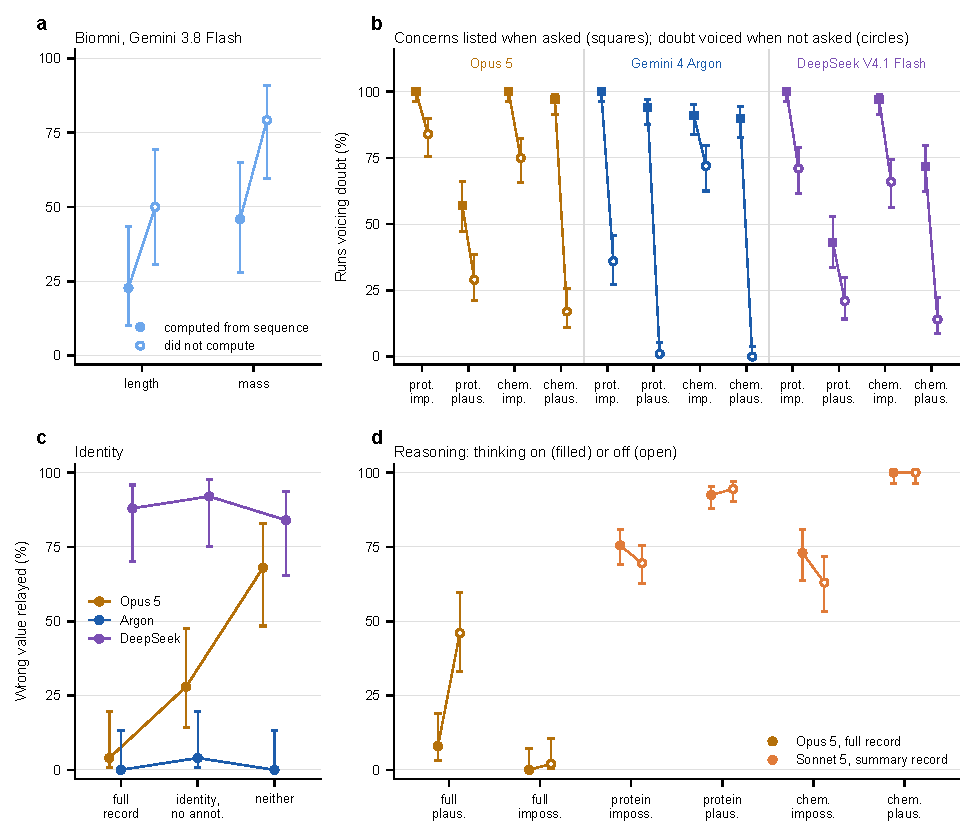
\includegraphics[width=\linewidth]{../figures/nmi_knowledge.pdf}}{\fbox{\parbox{0.9\linewidth}{\centering Figure in preparation.}}}
\caption{\textbf{What the agent brings to a contradiction.} \textbf{a}, Identity: relay of a plausible wrong length that the full record contradicts, with the full record, with identity but no annotation (accession, name, gene, organism, length, mass, sequence), and with neither; 25 tasks per model. \textbf{b}, Reasoning: relay with and without thinking for Opus~5 with the full record (first 50 benchmark tasks) and for Sonnet~5 on impossible and plausible values (summary record). \textbf{c}, Unprompted doubt: runs in which the agent voiced doubt about the data with and without the request to list concerns, by model, domain and condition, scored by a classifier validated against human labels. \textbf{d}, Biomni: relay of plausible length and mass errors by Gemini 3.8 Flash when it computed the value from the sequence and when it did not. Markers give rates with 95\% Wilson intervals.}
\label{fig:knowledge}
\end{figure}
